\documentclass[english]{article}

\usepackage{babel}
\usepackage{graphicx}
\usepackage{times}
\usepackage{pifont}
\usepackage[margin=1in]{geometry}
\usepackage{eurosym}
\usepackage{fancyhdr}
\usepackage[hidelinks]{hyperref}
\usepackage{listings}
\usepackage{color}
\usepackage{float}
\usepackage{listings}
\usepackage{caption}
\usepackage{subcaption}


\fancyhf{}


%HEADER
%**************************************************************************************
\pagestyle{fancy}
\fancyhf{}
%**************************************************************************************
\lhead{AD converter}		 	 
\rhead{Basics of Microprocessor technology} 
\lfoot{EFA12SF}
\cfoot{\thepage}
\rfoot{Nikolay Arsenov\\Alexey Tukalo}
%**************************************************************************************

\date{}
\setlength\parindent{0pt}

\begin{document}

\title{\vspace{2in}AD converter\\
\small for Basics of Microprocessor technology\\
\vspace{0.5in}
\includegraphics{savonia.jpg}}

\nopagebreak
\maketitle


\vspace{3in}

\author{
\begin{flushright}
Nikolay Arsenov,Alexey Tukalo,\\
EFA12SF,\\
Information Technology,\\
Savonia University of Applied Sciences
\end{flushright}
}

\date{\today}
\thispagestyle{empty}

\newpage
\setcounter{page}{1}
\setcounter{tocdepth}{2}
\tableofcontents

\newpage


\section{AD - converter}
An analog-to-digital converter (ADC, A/D, or A to D) is a device that converts a continuous physical quantity (usually voltage) to a digital number that represents the quantity's amplitude.
\subsection{List of Features•}
\begin{itemize}
\item 10-bit Resolution
\item 1 LSB Integral Non-linearity
\item ±2 LSB Absolute Accuracy
\item $13\mu s - 260 \mu s$ Conversion Time
\item Up to 76.9kSPS (Up to 15kSP S at Maximum Resolution)
\item 16 Multiplexed Single Ended Input Channels
\item 14 Differential input channels
\item 4 Differential Input Channels with Optional Gain of 10x and 200x
\item Optional Left Adjustment for ADC Result Readout
\item 0V – VCC ADC Input Voltage Range
\item 2.7V – VCC Differential ADC Voltage Range
\item Selectable 2.56V or 1.1V ADC Reference Voltage 
\item Free Running or Single Conversion Mode
\item Interrupt on ADC Conversion Complete
\item Sleep Mode Noise Canceler
\end{itemize}
\subsection{The main ATmega2560 features}
\paragraph{A 10-bit successive approximation ADC.} The ADC converts an analog input voltage to a 10-bit digital value through successive approximation.
\paragraph{A successive-approximation ADC} uses a comparator to successively narrow a range that contains the input voltage. At each successive step, the converter compares the input voltage to the output of an internal digital to analog converter which might represent the midpoint of a selected voltage range. At each step in this process, the approximation is stored in a successive approximation register (SAR). For example, consider an input voltage of 6.3 V and the initial range is 0 to 16 V. For the first step, the input 6.3 V is compared to 8 V (the midpoint of the 0–16 V range). The comparator reports that the input voltage is less than 8 V, so the SAR is updated to narrow the range to 0–8 V. For the second step, the input voltage is compared to 4 V (midpoint of 0–8). The comparator reports the input voltage is above 4 V, so the SAR is updated to reflect the input voltage is in the range 4–8 V. For the third step, the input voltage is compared with 6 V (halfway between 4 V and 8 V); the comparator reports the input voltage is greater than 6 volts, and search range becomes 6–8 V. The steps are continued until the desired resolution is reached.
\paragraph{16 Multiplexed Single Ended Input Channels.} The ADC is connected to an 8/16-channel Analog Multiplexer which allows eight/sixteen single-ended voltage inputs. The analog input channel is selected by writing to the MUX bits in ADMUX and ADCSRB. Any of the ADC input pins, as well as GND and a fixed bandgap voltage reference, can be selected as single ended inputs to the ADC. A selection of ADC input pins can be selected as positive and negative inputs to the differential amplifier. If differential channels are selected, the voltage difference between the selected input channel pair then becomes the analog input to the ADC. If single ended channels are used, the amplifier is bypassed altogether.
\paragraph{Four Differential Input Channels with Optional Gain of 10x and 200x.} The device also supports 16/32 differential voltage input combinations. Four of the differential inputs (ADC1 \& ADC0, ADC3 \& ADC2, ADC9 \& ADC8 and ADC 11 \& ADC 10) are equipped with a programmable gain stage, providing amplification steps of 0 dB (1x), 20 dB (10x) or 46 dB (200x) on the differential input voltage before the ADC conversion. The 16 channels are split in two sections of 8 channels where in each section seven differential analog input channels share a common negative terminal (ADC1/ADC9), while any other ADC input in that section can be selected as the positive input terminal. If 1x or 10x gain is used, 8 bit resolution can be expected. If 200x gain is used, 7 bit resolution can be expected.
\paragraph{Selectable 2.56V or 1.1V ADC Reference Voltage.} Internal reference voltages of nominally 1.1V, 2.56V or A VCC are provided On-chip. The voltage reference may be externally decoupled at the AREF pin by a capacitor for better noise performance. The minimum value represents GND and the maximum value represents the voltage on the AREF pin. Optionally, AVCC or an internal reference voltage (1,1V or 2,56V) may be connecter to the AREF pin by writing to the REFSn bits in the ADMUX Register that can help to improve noise immunity.
\paragraph{Interrupt on ADC Conversion Complete.} The ADC has its own interrupt which can be triggered when a conversion completes.\\\\
The ADC contains a Sample and Hold circuit which ensures that the input voltage to the ADC is held at a constant level during conversion. A block diagram of the ADC is shown in Figure 1.
\begin{figure}[H]
\centerline{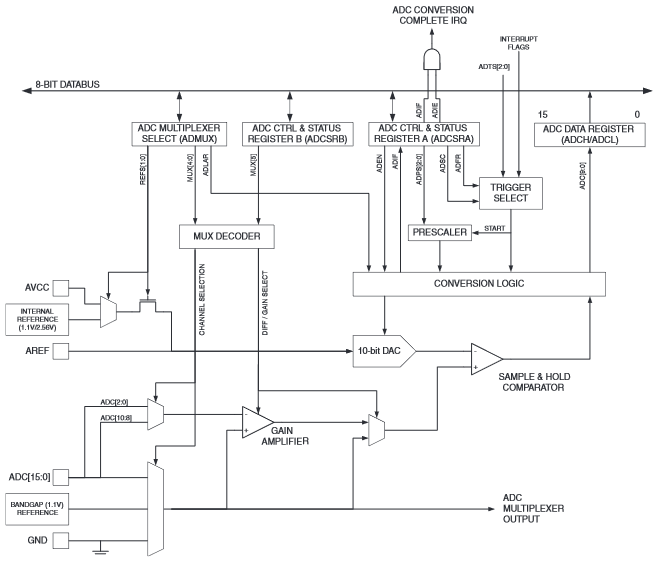
\includegraphics[scale=0.8]{MicroLab8/1}}
\caption{Analog to Digital Converter Schema}
\end{figure}
\section{Controlling the conversion frequency}
Before using the ADC it is necessary to select the reference voltage source and the ADC clock frequency. The voltage reference source options (Figure 2) can be determined by setting certain bits 6 and 7 in the ADCMUX register shown in Figure 3.
\begin{figure}[H]
\centerline{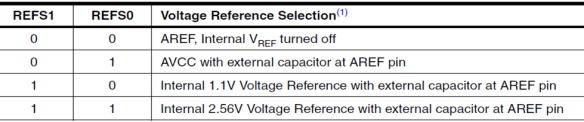
\includegraphics[scale=0.8]{MicroLab8/2}}
\caption{ADC reference voltage source}
\end{figure}
\begin{figure}[H]
\centerline{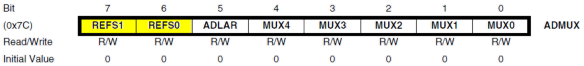
\includegraphics[scale=0.8]{MicroLab8/3}}
\caption{ADC multiplexer register, showing the reference source bits}
\end{figure}
The ADC can be operated in the following three modes: 
\begin{itemize}
\item Single conversion: Started by writing a logical one to the ADC Start Conversion bit
\item Triggered conversion: The conversion is initiated by the rising edge of the trigger input
\item Free running: The next conversion takes place immediately after the previous conversion is finished
\end{itemize}
The ADC prescale controls the internal ADC clock that controls the conversion process. By default, the successive approximation circuitry requires an input clock frequency between 50kHz and 200kHz. If a lower resolution than 10 bits is needed, the input clock frequency to the ADC can be as high as 1000kHz to get a higher sample rate. The conversion process requires 13-14 ADC clock cycles and this sets an upper limit on the sampling frequency. The pre-scale options are shown in Figure 4.
\begin{figure}[H]
\centerline{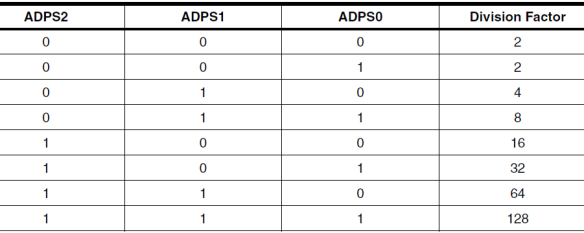
\includegraphics[scale=0.8]{MicroLab8/4}}
\caption{ADC prescale values}
\end{figure}	
The certain prescale value will give ADC clock frequency. For example, when we use a 16MHz oscillator then use a prescale value of 128 (taken from the Figure 4) will give ADC clock frequency of 125kHz (see a equation below) which is well within the 50kHz and 200kHz limits.\\\\
16MHz/128 = 125kHz the ADC reference clock
\begin{itemize}
\item 16 MHz / 2 = 8 MHz
\item 16 MHz / 4 = 4 MHz
\item 16 MHz / 8 = 2 MHz
\item 16 MHz / 16 = 1 MHz
\item 16 MHz / 32 = 500 kHz
\item 16 MHz / 64 = 250 kHz
\item 16 MHz / 128 = 125 kHz
\end{itemize}
It is also necessary to carry out a single conversion by setting the ADSC bit in the ADCSRA register \begin{figure}[H]
\centerline{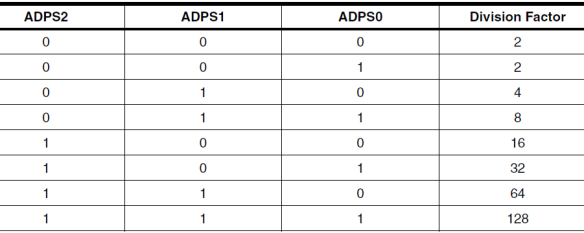
\includegraphics[scale=0.8]{MicroLab8/4}}
\caption{ADC Control and Status Register, with clock prescale bits highlighted}
\end{figure}
Setting bits happens by using command below (as an example 128 prescale value):
$ADCSRA |= ((1<<ADPS2) | (1<<ADPS1) | (1<<ADPS0))$;
A normal conversion in the ADC takes 13 ADC clock cycles. The first conversion takes 25 clock cycles (see Figure 6).
\begin{figure}[H]
\centerline{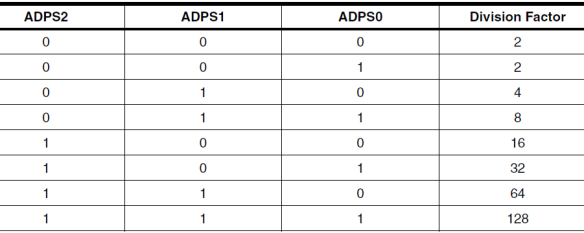
\includegraphics[scale=0.8]{MicroLab8/4}}
\caption{ADC Conversion Time}
\end{figure}
So our ADC clock speed needs to be factored down by 13 to figure out how many samples we will be able to achieve per second. The Arduino library is enabling the ADC with a 128 prescaler, giving a 125 kHz ADC clock speed when the core clock is 16 Mhz. A 125 kHz clock speed will result in 125 kHz / 13 = 9600 Hz sample speed. The hardware limit is 9,600 samples per second or 96 samples per millisecond. We cannot physically do better than that at the desired 10 bit resolution. As we can see, we got 9600Hz sample speed, it is the same value, which we will use in our programming tasks.
\section{Changing the input voltage}
Once the ADC is initialised single conversions on any channel are carried out by first selecting the desired channel, it is starting the conversion by writing a logical one to the ADC Start Conversation bit, ADSC. It named “the conversion complete flag” (ADSC bit in the ADCSRA register, shown in figure 5). Until the conversion is complete ADSC=1 and stays high as long as the conversation is in progress and will be set to ADSC=0 when the conversion is complete, will be cleared by hardware. Then finally it will read the converted value. If a different data channel is selected while a conversation is in progress, the ADC will finish the current conversation before performing the channel change.\\\\
Alternatively, a conversion can be triggered automatically by Auto Triggering, which can be enabled by setting the ADC Auto Trigger Enable bit, ADATE in ADCSRA. When a positive edge occurs on the selected trigger signal, the ADC prescaler is reset and a conversion is started. This provides a method of starting conversions at fixed intervals. If the trigger signal still is set when the conversion completes, a new conversion will not be started. If another positive edge occurs on the trigger signal during conversion, the edge will be ignored.\\\\
If we would like to measure input signals using differential channels, the certain type of conversion should be taken into consideration. We will use differential conversions that are synchronized to the internal clock. A conversion initialed that there are all single conversions, and the first is free running conversion. So, when the clock is low will take the same amount of time as a single ended conversion (13 ADC clock cycles), if we will have another conversion with another signal, the clock will be high and will take more time due to the synchronization mechanism (14 ADC clock cycles).
\section{The scaling of the result}
After the conversion is complete (ADIF is high), the conversion result can be found in the ADC\\\\ Result Registers (ADCL, ADCH).\\\\
For single ended conversion, the result is:
$$
ADC=\frac{V_{IN}\cdot 1023}{V_{REF}}
$$
Because of we have 10-bit resolution, we have $2^{10}=1024$ possible values for each analog value in the rage $(0-V_{REF})$ Volts we have $(0 - 1023)$ decimals numbers.\\\\
In this equation $V_{IN}$ means the voltage on the selected pin (Analog input pins) and $V_{REF}$ is selected reference voltage (1.1V or 2.5V), depends on the programmed registers. For example: If we have input constant voltage taken from the power supply equals 1V and reference voltage chosen 2.5V in this case ADC output will be:
$$
ADC=\frac{1V \cdot 1023}{2.5V}=\frac{1023}{2.5}=409.2
$$
ADC output presented in decimal number is 409.2. This is a digital number, which we can get from the AVR microcontroller on the desktop PC.\\\\
If differential channels are used, the result is:
$$
ADC=\frac{(V_{POS}-V_{NEG})\cdot Gain \cdot 1023}{V_{REF}}
$$
In this equation $V_{POS}$ means positive voltage, $V_{NEG}$ is negative voltage are two differential input channels, Gain can be selected as 1x,10x or 200x and $V_{REF}$ is selected reference voltage (1.1V or 2.5V), depends on the programmed registers.
\section{Programming the circuit}
Usually, to make programming easier, programmers creates a separate method for initializing necessary variables or to program necessary registers for microcontroller’s bits.
\begin{figure}[H]
\centerline{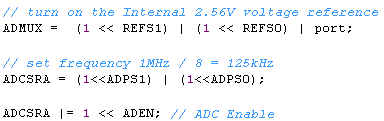
\includegraphics[scale=0.8]{MicroLab8/7}}
\caption{Example of a method called Init\_ADC}
\end{figure}
Here we have a peace of code, which gives certain values to registers important for us. In ADMUX – multiplexer register we can first of all choose the internal reference voltage for measurements, by setting values to pins (REFS1 and REFS2), or we can switch on/off MUXn (MUX0, MUX1,  MUX2, MUX3, MUX4) to read bits from new channels see Figure 7 below. \\\\
$ADMUX = (1<<MUX0) | (1<<MUX3)$ means we set our mux into position 4, to work with ADC channel number three to read analog input from ADC3 and convert it to the digital signal.\\\\
ADCSRA give us an opportunity to program the conversion frequency by setting bits into ADPS1, ADPS2 and ADPS3 according Figure 5. Also we can enable and disable ADC in our microcontroller by setting value into ADEN register. Others programming principles will be shown in the programming exercises below.
\begin{figure}[H]
\centerline{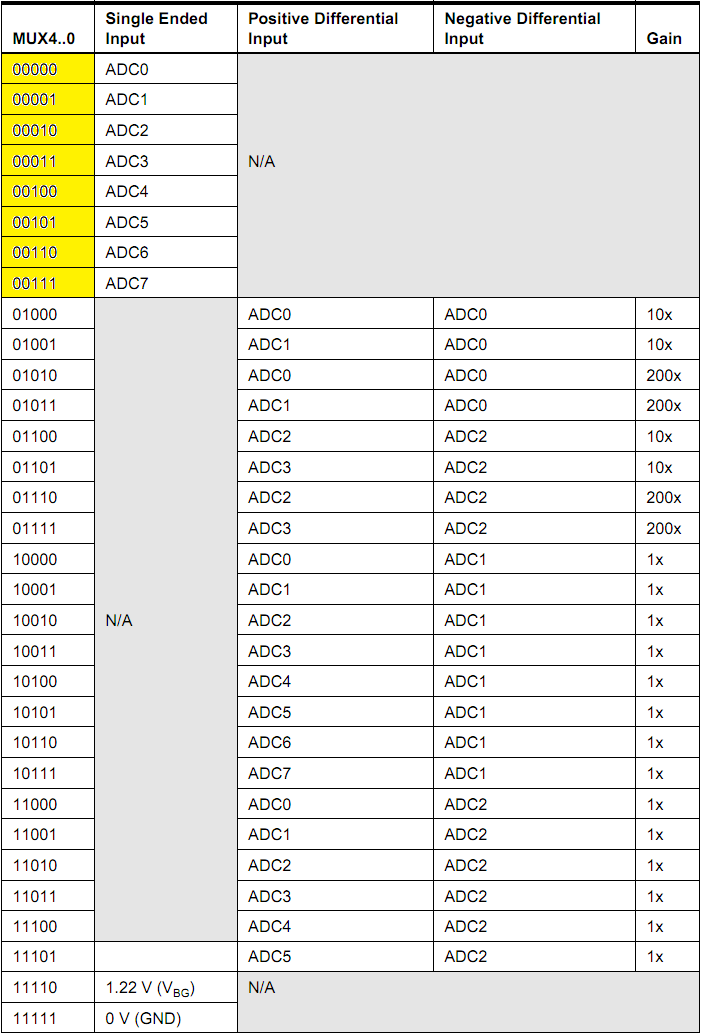
\includegraphics[scale=0.8]{MicroLab8/MUXn}}
\caption{Example of a method called Init\_ADC}
\end{figure}
\section{Programming tasks}

\subsection{The first task}
\lstinputlisting[caption=L8\_1.c]{MicroLab8/L8_1.c}
\lstinputlisting[caption=main.c]{MicroLab8/main1.c}

\subsection{The second task}
\lstinputlisting[caption=L8\_2.c]{MicroLab8/L8_2.c}
\lstinputlisting[caption=main.c]{MicroLab8/main2.c}

\subsection{The third task}
\lstinputlisting[caption=L8\_3.c]{MicroLab8/L8_3.c}
\lstinputlisting[caption=main.c]{MicroLab8/main3.c}
\subsection{The fourth task}
\lstinputlisting[caption=L8\_4.c]{MicroLab8/L8_4.c}
\lstinputlisting[caption=main.c]{MicroLab8/main4.c}
ADC0, ADC1 are Grounded; ADC2, ADC3 have voltages from the power source and the rest ADCs pins are not grounded, that’s why they have value equals to Vref.
\begin{figure}[H]
\centerline{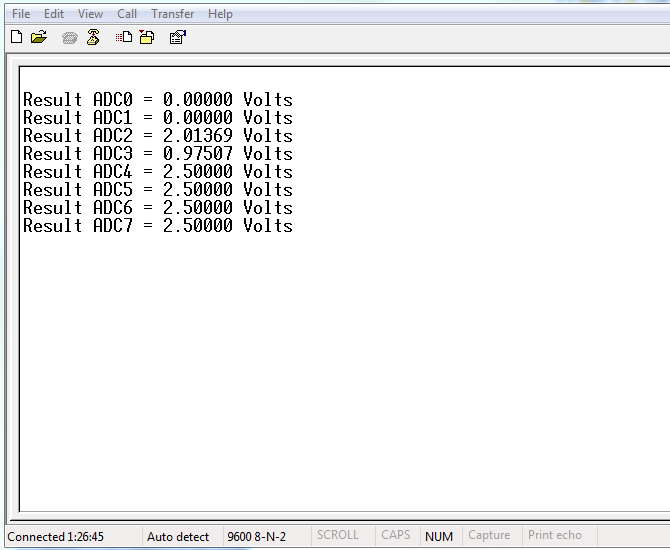
\includegraphics[scale=0.8]{MicroLab8/1r}}
\caption{Results of the measurement}
\end{figure}
We can change inputs values during 10 seconds no changes will be shown, but after 10 seconds new values will be shown in the terminal. ADC0, ADC3 are Grounded; ADC1, ADC2 have voltages from the power source and the rest ADCs pins are not grounded, that’s why they have value equals to Vref.
\begin{figure}[H]
\centerline{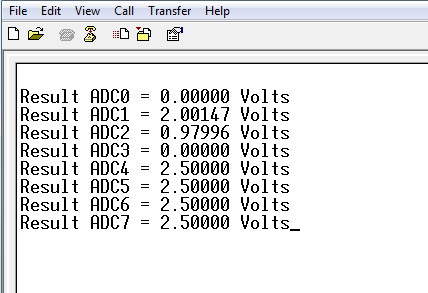
\includegraphics[scale=0.8]{MicroLab8/2r}}
\caption{Results of the measurement}
\end{figure}
\end{document}
